% 第三问：风格生成与迁移可行域

\section{第三问：风格生成与迁移可行域}\label{sec:q3}

第三问要做两件性质不同的事：在给定风格下生成新的化合物—感官谱，以及判断一款现有酒能否改造成目标风格。本文把二者拆成生成层与判别层：生成层回答哪种采样最像真实酒，判别层回答哪条改造路径在化学上站得住。总的判断是，生成质量无法用单一指标排序；迁移可行域主要由 DMS 与反式-2-壬烯醛卡住，且对阈值高度敏感。

\subsection{风格条件生成与评价体系}

生成质量在不同评价维度上会给出相反的排序，因此本文的生成体系从一开始就把分布接近与分类器认可分开记录。三个角色的划分互不重叠，是为了让生成器用过的酒不出现在评价里：生成器只用 G，评价器只用 J，真实参考只用 T。同一批 250 款酒在五次划分中被重复使用，因此后文的比较都是划分内比较，不构成外部验证。

生成对象取 Tripel（28 款）、Kriek（10 款）与 Lambic（11 款）。前者的样本量足以支撑 40 条谱的分布比较，后两者稀少，正好用来观察少样本风格上的退化；三个风格的样本量跨度覆盖了够用与不够用两种情形。每次划分把 250 款酒分成互不重叠的 G（生成器训练，100 款）、J（评价器训练，100 款）与 T（留出检验，50 款）；四种方法在每种风格上各生成 40 条谱，五次划分合计 2400 条。生成器只看到 G 中该风格酒样的 226 个非聚合化学字段。Kriek 与 Lambic 每划分进入 G 的只有 4 至 5 款、进入 T 的真实参考只有 2 款，Tripel 则为 11 款与 6 款，这一不对称决定了后文的读数方式。

四种方法对应四种关于配方空间的假设。重采样有放回地抽取 G 中的同风格酒样，不学习任何结构，是必须被击败的基线\cite{efron1993}；它不产生新组合，却是唯一保证生成点落在真实数据流形上的方法，任何生成器若在分布距离上赢不过它，就说不上学到了结构。局部凸组合假定新配方落在同风格近邻的连线上：
\begin{equation}
x_{\mathrm{new}}=u\,x_{a}+(1-u)\,x_{b},\qquad 0\le u\le 1,
\label{eq:convex}
\end{equation}
其中 $x_a,x_b$ 为 G 中同风格的两个酒样。凸组合对应配比微调这一工艺动作，生成点不会超出数据支撑。受约束局部凸组合在 \eqref{eq:convex} 之上要求生成点到最近同风格训练样本的距离不超过留一支撑半径，并在对数尺度上混合 DMS 与 4VG、裁剪到上下界。条件 PCA 高斯在 G 的风格内做主成分分解后于主成分空间拟合对角高斯并采样，允许生成点离开凸包，更容易产生训练集中没有的组合。

评价从生成器外部取四个角度。分布距离用固定训练带宽的 RBF 核最大均值差异 $\mathrm{MMD}^2$\cite{gretton2012}，真实参考为 T 中该风格酒样的非缺失测量；KS 统计量逐字段计算后取均值，刻画边缘分布的平移；精确复制比例统计与 G 中某训练点距离小于 $10^{-8}$ 的生成谱占比；独立评价器是只在 J 上训练的风格分类器，报告它赋予目标风格的平均概率与判为目标风格的比例。四项指标共用同一套预处理与核带宽，尺度差异不会被误读成分布差异。KS 只看单字段的边缘分布，对字段之间的相关性不敏感；$\mathrm{MMD}^2$ 在多维表示上一次比较整个联合分布，两者一起看才能区分单字段偏移与整体结构偏移。

分类器识别率高与分布更接近是两件不同的事。分类器只关心生成点落在决策边界哪一侧，对风格内部的协方差、尾部厚度与稀有组合不敏感；$\mathrm{MMD}^2$ 关心整个分布在再生核空间中均值嵌入的位置，对生成物挤向风格中心这类退化格外敏感。一种方法完全可以把样本堆到最典型的 Tripel 附近换来高识别率，同时因丢掉离散度而让 $\mathrm{MMD}^2$ 变大。本文因此不设综合评分，只并列报告四个维度。

\subsection{生成结果}

四种方法在三个风格上互有胜负，没有一种全面占优；重采样在分布距离上仍是难以击败的基线，但它的精确复制比例恒为 1。

\begin{table*}[t]
\centering
\caption{三种风格下四种生成方法的分布距离、边缘偏移、复制比例与独立评价器判断（五次划分平均；$\mathrm{MMD}^2$ 与 KS 越小越好，复制率为与训练点完全重合的生成谱比例，后两列由只在 J 上训练的分类器给出）}
\label{tab:gen}
\small
\begin{tabular}{llrrrrr}
\toprule
风格 & 方法 & $\mathrm{MMD}^2$ & KS 均值 & 复制率 & 评价器概率 & 判为目标风格 \\
\midrule
Tripel & 重采样 & 0.1034 & 0.4245 & 1.00 & 0.2992 & 0.565 \\
       & 局部凸组合 & 0.1135 & 0.4448 & 0 & 0.3432 & 0.755 \\
       & 受约束局部凸组合 & 0.1158 & 0.4463 & 0 & 0.3358 & 0.695 \\
       & 条件 PCA 高斯 & 0.1088 & 0.4605 & 0 & 0.1499 & 0.285 \\
\midrule
Kriek  & 重采样 & 0.2871 & 0.6208 & 1.00 & 0.5275 & 0.800 \\
       & 局部凸组合 & 0.3005 & 0.6511 & 0 & 0.5779 & 0.955 \\
       & 受约束局部凸组合 & 0.2988 & 0.6422 & 0 & 0.5703 & 0.950 \\
       & 条件 PCA 高斯 & 0.2832 & 0.6307 & 0 & 0.3101 & 0.595 \\
\midrule
Lambic & 重采样 & 0.2226 & 0.6257 & 1.00 & 0.4924 & 0.885 \\
       & 局部凸组合 & 0.2206 & 0.6602 & 0 & 0.5543 & 0.975 \\
       & 受约束局部凸组合 & 0.2181 & 0.6453 & 0 & 0.5598 & 0.995 \\
       & 条件 PCA 高斯 & 0.2095 & 0.6324 & 0 & 0.2091 & 0.385 \\
\bottomrule
\end{tabular}
\end{table*}

表\ref{tab:gen} 汇总五次划分的平均结果。Tripel 上受约束局部凸组合的识别率 0.3358 高于重采样的 0.2992，判为 Tripel 的比例 0.695 也高于 0.565，但它的 $\mathrm{MMD}^2$ 为 0.1158、KS 均值 0.4463，两项都劣于重采样的 0.1034 与 0.4245。同一风格上出现了方向相反的评价：按判别边界看受约束凸组合更像目标风格，按分布看重采样离真实酒样更近。重采样在两个距离指标上同时最好，说明它逼近真实分布靠的是直接复制，而不是学到了结构。约束没有换来指标收益，无约束版本的 $\mathrm{MMD}^2$ 为 0.1135、识别率 0.3432，两项都略好；约束的作用是保证生成谱不越界。

反向的例子同样清楚。条件 PCA 高斯在 Tripel 上的 $\mathrm{MMD}^2$ 为 0.1088，仅次于重采样，但独立评价器给它目标风格的概率只有 0.1499、判为目标风格的比例 0.285，两项都最低。这可能与对角高斯忽略主成分之间的相关性、生成点向风格中心收缩有关，结果是谱形趋于平均、反而越过分类边界。距离近而识别率低与识别率高而距离远，指向同一件事：两个指标度量的不是同一个东西。

Kriek 与 Lambic 上的距离整体大了一倍，落在 0.21 至 0.30 之间，四种方法都没有把这两个稀薄风格学到可用程度，而每划分只有 2 款留出酒，抽样误差不可忽略。这两个风格的化学谱离散度大、样本又少，40 条生成谱难以覆盖其变异范围。KS 在 Tripel 上集中在 0.42 至 0.46，在 Kriek 与 Lambic 上集中在 0.62 至 0.66；逐字段取平均会稀释单字段的尾部偏离，因此 KS 更适合判断整体平移，不适合判断尾部风险。Kriek 上条件 PCA 高斯最低（0.2832），重采样 0.2871；Lambic 上条件 PCA 高斯 0.2095、受约束凸组合 0.2181、重采样 0.2226，三者相差不足 0.014，识别率却相反，条件 PCA 高斯只有 0.2091。这两个风格上的读数只能支持重采样没有被稳定击败，不能支持任何方法的优越性。

覆盖度从另一侧约束生成质量。对每个真实酒样，计算它到最近生成点的标准化欧氏距离，再除以它到最近真实酒样的距离，得到相对覆盖比；比值小于 1 说明生成集把真实样品包住了。重采样最小（0.60--0.70），两种凸组合居中（0.61--0.73），条件 PCA 高斯最差（0.87--0.93），见表\ref{tab:coverage}。这解释了第二节的悖论：条件 PCA 高斯在 Kriek 与 Lambic 上 $\mathrm{MMD}^2$ 最低，并不是更贴近真实酒样，而是生成点偏离训练支撑、把分布拉宽，因而在核均值嵌入上"看起来"更接近。三项指标合起来才有完整判断：重采样保真且覆盖最好，但复制率为 1、不产生新组合；凸组合产生新组合、覆盖尚可，分布距离略差；条件 PCA 高斯覆盖最差。

\begin{table}[t]
\centering\small\renewcommand{\arraystretch}{1.15}
\caption{生成集的相对覆盖比（真实酒样到最近生成点距离 / 到最近真实酒样距离）}
\label{tab:coverage}
\begin{tabular}{@{}lccc@{}}
\toprule
方法 & Tripel & Kriek & Lambic \\
\midrule
重采样 & 0.698 & 0.653 & 0.600 \\
局部凸组合 & 0.729 & 0.648 & 0.606 \\
受约束局部凸组合 & 0.711 & 0.655 & 0.634 \\
条件 PCA 高斯 & 0.919 & 0.874 & 0.933 \\
\bottomrule
\end{tabular}
\end{table}

复制率给出了最干净的分界：重采样恒为 1，两种凸组合与条件 PCA 高斯恒为 0。复制率为 1 意味着每条生成谱都是训练集中已有的酒，作为生成新配方没有提供新组合，这正是重采样距离更近却不适合交付的原因。凸组合的复制率为 0，说明它们给出的是新的配比组合，代价是可能落在真实酒样稀疏的区域。

\begin{figure*}[t]
\centering
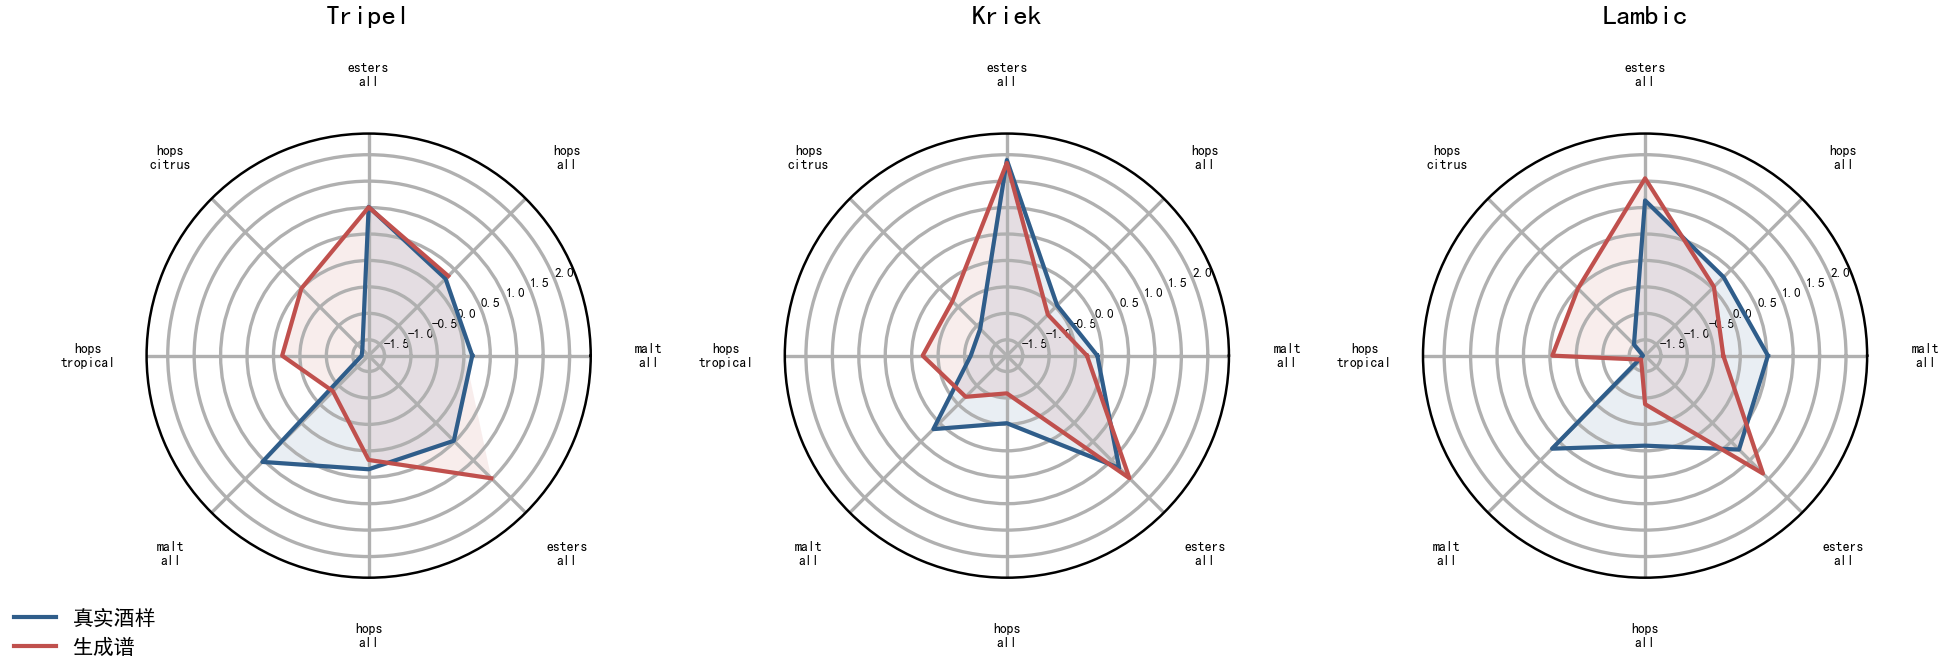
\includegraphics[width=0.98\textwidth]{figures/fig11_generation.png}
\caption{三种风格的真实酒样与生成谱在 8 个标准化感官维度上的相对强度。纵轴为按 8 维标准化后的相对强度，可正可负，因此比较的是曲线形状而不是绝对得分；生成谱的感官画像由第一问的预测模型给出，是预测值而非新酿酒的实测评价。}
\label{fig:gen}
\end{figure*}

图\ref{fig:gen} 的曲线在形状上大体重合，没有整体平移或维度错位，差异集中在酒花与麦芽两族维度，说明凸组合把邻近样本的谱形带了进来。

\subsection{迁移搜索与冻结候选}

迁移的可行性在三个证据层级上依次衰减，搜索可行只是最弱的一层。

迁移任务给定一款 Pils/Lager 源酒，问能否通过调整配比把它推到 Tripel。候选由源酒与 G 内每个 Tripel 锚点之间的线性插值生成，每个锚点取 30 档权重，逐点裁剪回给定上下界；每条记录由此产生 30 档乘锚点数的候选，绝大多数会在下一步被淘汰。筛选条件有五条：标准化空间的均方根改动不超过半径 1；到最近 Tripel 训练点的距离不超过其留一支撑半径；目标风格概率不低于 0.5，且比源酒与仅裁剪对照高出 0.01；四项缺陷不增；两个 G 感官模型给出的 stale hops 代理不增。

半径按标准化特征的均方根改动计量，半径 1 约等于各字段平均改动一个标准差，属于配方微调的量级。半径 0.25、0.5、1、2 都跑过；半径变大时，候选更多，但改动也更大，本文只报告半径 1，其余半径用于检查结论是否随半径翻转。通过的候选再按改动量、目标距离与已知阈值超额做 Pareto，取改动最小者，以免为了风格标签牺牲过多化学余量。半径之外的候选不进入排序，因此本文报告的是在可接受改动内能做到什么，而不是最优改动有多大。

搜索模型使用G训练，候选冻结后用J训练的模型复核；T是从同一历史数据集中划出的内部留出酒。全部来源结果包含G、J和T来源，其中J来源酒参与了J模型训练；仅T来源在两类模型训练之外，仍不是新的外部样本。半径 1 下 55 条来源与划分的组合记录（11 款 Pils/Lager 源酒乘 5 次划分）见表\ref{tab:transfer}。

\begin{table}[t]
\centering
\caption{半径 1 下迁移候选的三级通过情况（55 条来源与划分记录；后三列依次为 G 搜索可行、J 独立代理支持、以及在原始 0--6 尺度上 stale hops 代理同样不增）}
\label{tab:transfer}
\small
\setlength{\tabcolsep}{1pt}
\begin{tabular}{lrrrr}
\toprule
记录集 & 条数 & G 可行 & J 支持 & 原始尺度后 \\
\midrule
全部来源 & 55 & 51 & 11 & 6 \\
其中 T 留出（7 款酒） & 10 & 10 & 2 & 1 \\
\bottomrule
\end{tabular}
\end{table}

G 上 55 条中有 51 条找到可行候选，换到 J 的独立模型后只剩 11 条，补上原始 0--6 尺度的 stale hops 不增后只剩 6 条。T 留出的 10 条记录（7 款酒）在同样三级口径下依次为 10、2、1。第一段衰减最大：G 的锚点与源酒共享训练信息，分类器判断偏乐观，换成 J 就掉了 40 条。第二段来自尺度：J 在标准化空间里的代理与原始尺度上的预测并不等价，补上一条后又有 5 条落选。T 的10条记录均在G上找到候选，其中1条通过全部代理条件；该组只有7款不同来源酒，不能据此确认训练来源与留出来源具有相同性能。

结论是，搜索可行不等于代理支持，代理支持也不等于真实品评。三层证据的强度依次递增，只能分层报告；把 51 读成 51 款酒改造成功，等于把跨模型的一致性问题当成实验结果。找不到候选时保留源酒并记录失败，不把源酒当作可行解。stale hops 是第一问模型对老化酒花的预测分，它的不增只表示两个模型在这一点上不矛盾，不构成感官实测。

\subsection{严格浓度约束与不可行证书}

在逐项浓度不增的严格协议（下称协议 A）下，55 条记录的最大 Tripel 份额全部为 0，且每一条都附带可验证的不可行证书；这把无解从数值结果变成了可定位到具体化合物的工艺诊断。

混配只使用 61 个有单位、有报告值的浓度字段，其余字段只有对数化的相对值，无法进入按质量守恒写出的混配式。以某款 Pils/Lager 为基液、G 中的 Tripel 酒样为锚点，混配后的浓度为
\begin{equation}
c(w)=c_{0}+\sum_{j=1}^{m}w_{j}\,(c_{j}-c_{0}),
\label{eq:mix}
\end{equation}
\eqref{eq:mix} 中的 $c_0$ 为源酒浓度向量，$c_j$ 为第 $j$ 个锚点的浓度向量，$w_j\ge 0$ 为 Tripel 的添加份额，剩余 $1-\mathbf{1}^{\mathsf T}w$ 为源酒。四项缺陷逐项不增的要求给出线性规划
\begin{equation}
\begin{aligned}
\max_{w}\ &\mathbf{1}^{\mathsf T}w\\
\mathrm{s.t.}\ \ &Mw\le 0,\quad w\ge 0,\quad \mathbf{1}^{\mathsf T}w\le 0.75,
\end{aligned}
\label{eq:lp}
\end{equation}
$M$ 的第 $(d,j)$ 元为 $c_{j,d}-c_{0,d}$，份额上界 0.75 对应以现有酒为主体、只做局部调整；该上界是本文设定的搜索约束，0.75 本身不保证成品保留来源酒的工艺或身份。最优值同时是可行性判据：为正，就存在一条提高 Tripel 份额的配比；为 0，说明这个方向上没有任何余量。55 条记录在 \eqref{eq:lp} 下的最优值全为 0，即任何正份额的 Tripel 添加都会使至少一项缺陷高于源酒。

无解本身不算结论，能指出被谁挡住才算。对每条记录求解一个对偶证书：存在 $v\ge 0$ 使
\begin{equation}
\left(M_{\mathrm{norm}}^{\mathsf T}v\right)_{j}>0,\qquad j=1,\dots,m,
\label{eq:cert}
\end{equation}
其中 $M_{\mathrm{norm}}$ 按行最大值归一化，用于消除四项缺陷的量纲差异；按行归一化只改变每项缺陷的尺度，不改变不等号方向，因此证书的结论与原尺度上的线性规划一致。证书的本质是给出一组非负权重，使按该权重加权的四项缺陷偏离在任何正份额下都为正。若 \eqref{eq:cert} 成立，则任意 $w\ge 0$、$w\ne 0$ 有 $v^{\mathsf T}M_{\mathrm{norm}}w=\sum_{j}(M_{\mathrm{norm}}^{\mathsf T}v)_{j}w_{j}>0$，而 $M_{\mathrm{norm}}w\le 0$ 在 $v\ge 0$ 下又要求该内积非正，矛盾，故正份额不可行。55 条记录全部找到这样的证书，归一化余量 $\min_{j}(M_{\mathrm{norm}}^{\mathsf T}v)_{j}$ 介于 0.0002 与 0.2323 之间，中位数 0.1094。余量越小，约束越贴身。

消融把结论落到化合物上。逐个删除四项约束后，允许正份额的记录数分别为 30、4、0、4 条，对应删除 DMS、双乙酰、4VG 与反式-2-壬烯醛。删 4VG 一条也没有放开，说明它从不单独构成阻塞。按阻塞结构归类，DMS 单独阻塞 14 条、壬烯醛单独阻塞 15 条、两者联合阻塞 6 条、双乙酰 4 条，另有 16 条必须同时放松多项约束才能放开。配方调不动由此变成一句可执行的工艺语言：先把 DMS 与壬烯醛通路降下来，再谈风格迁移。

\subsection{阈值风险协议与联合复核}

可行域对缺陷阈值的取值极其敏感，把阈值写成可调参数而不是常数，才是可检验的做法。

题面要求的是超阈值项不恶化，而 \eqref{eq:lp} 的协议 A 要求逐项浓度不增，比题意强得多。协议 A 先于协议 B 被采用，是因为它不需要阈值，只依赖测量本身。协议A要求全部四项浓度不超过来源；协议B在来源低于阈值时允许浓度上升到阈值，在来源高于阈值时要求浓度不超过来源。为此定义风险函数
\begin{equation}
R_{d}(c)=\max\left(\frac{c}{t_{d}}-1,\ 0\right),
\label{eq:risk}
\end{equation}
按 \eqref{eq:risk} 的定义，协议 B 要求 $R_{d}(c')\le R_{d}(c)$，等价于 $c'\le\max(c,t_{d})$：低于阈值时以阈值为界，高于阈值时以原值为界。参考阈值取 DMS $19\ \mu$g/L、双乙酰 0.09 mg/L、4VG 0.2 mg/L（均取 8.xlsx 对应字段阈值的中位数）与反式-2-壬烯醛 $0.1\ \mu$g/L（8.xlsx 无该字段阈值，取文献值\cite{meilgaard1993,santos2003}）。中位数混合了不同基质与前处理方法，只能当作数量级参考。

\begin{table}[t]
\centering\small
\caption{四项化学风险的参考阈值来源}\label{tab:defectthreshold}
\begin{tabular}{@{}p{.30\columnwidth}p{.22\columnwidth}p{.38\columnwidth}@{}}
\toprule
字段 & 参考阈值 & 来源及基质\\
\midrule
DMS & 19 $\mu$g/L & 附件8阈值中位数；基质混合\\
双乙酰 & 0.09 mg/L & 附件8阈值中位数；基质混合\\
4VG & 0.20 mg/L & 附件8阈值中位数；基质混合\\
反式-2-壬烯醛 & 0.1 $\mu$g/L & 啤酒文献参考\cite{meilgaard1993,santos2003}\\
\bottomrule
\end{tabular}
\end{table}

这四项是浓度代理，stale hops 另由历史面板均分预测；附件中三项中位数的原始测量基质不统一，不能视作待制备批次的标定阈值。文献的0.1 $\mu$g/L适用于所述啤酒品评与老化分析条件，个体和基质差异仍需要测量确认。


将四个阈值统一乘以 0.5、1、2 后重解 \eqref{eq:lp} 并施加协议 B，允许正份额的记录数为 15、30、34。阈值收紧一半会把可行记录压到不足三分之一，放宽一倍却只多放开 4 条。图\ref{fig:feas} 把化学可行与代理复核两层放在一起。以1倍参考阈值为主要分析口径，0.5倍和2倍仅用于考察阈值设定的敏感性。

\begin{figure*}[t]
\centering
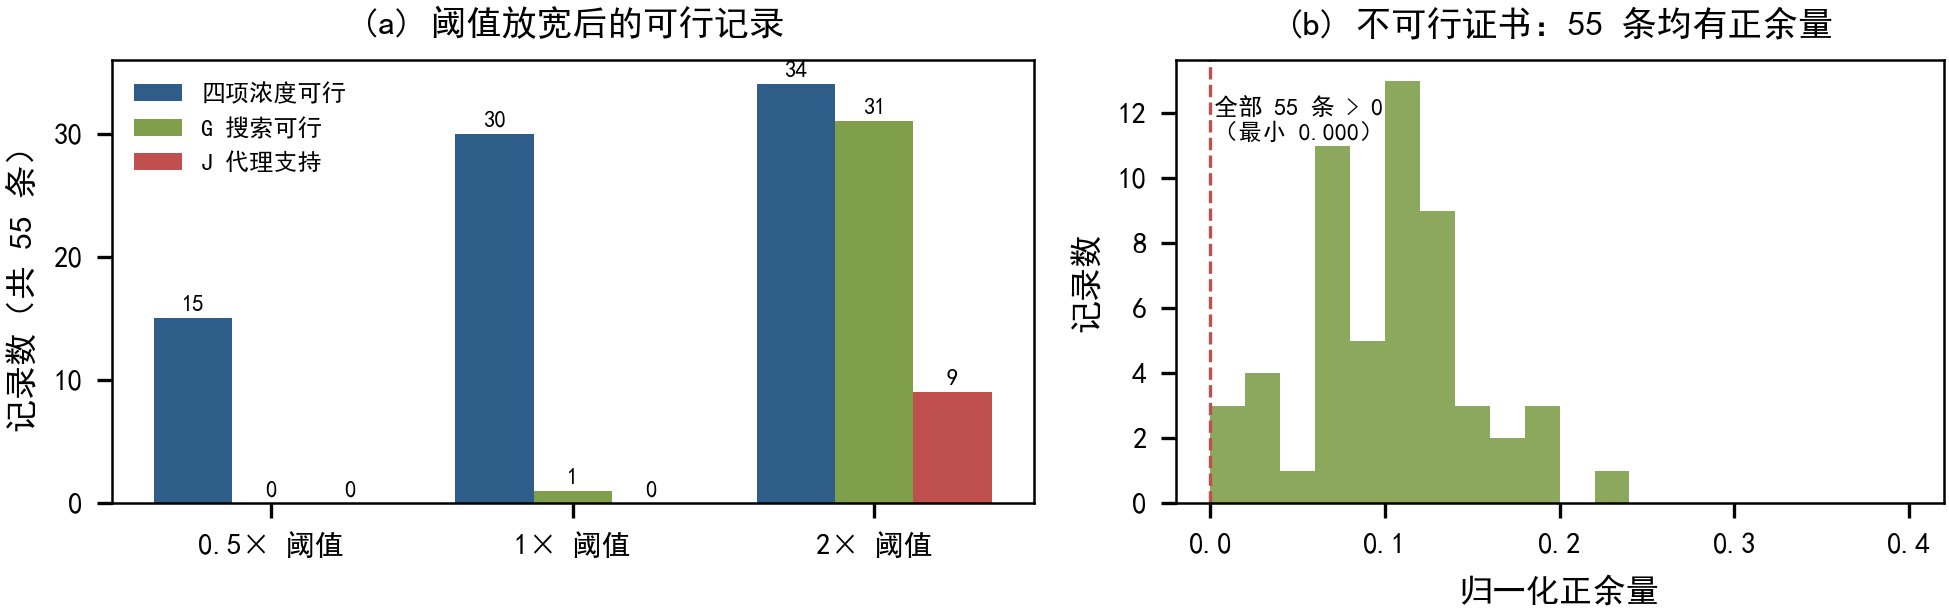
\includegraphics[width=0.98\textwidth]{figures/fig12_feasible.png}
\caption{(a) 缺陷阈值取 0.5 倍、1 倍、2 倍时，55 条记录中四项浓度可行、G 上搜索可行与 J 代理支持的条数；(b) 55 条不可行证书的归一化余量分布，全部大于 0。左图显示可行条数随阈值放宽而非线性增长，右图显示每条不可行记录都带正余量，即无解是结构性的而非求解失败。}
\label{fig:feas}
\end{figure*}

在化学可行的记录上叠加风格与 stale hops 约束，三层漏斗在 0.5 倍、1 倍、2 倍阈值下依次为：G 找到 0、1、31 条候选，J 复核后剩 0、0、9 条。阈值放宽到 2 倍时化学可行 34 条，其中 31 条能在 G 上找到风格候选，最终只剩 9 条通过 J，落差主要发生在代理层而不是化学层。联合复核把化学可行、风格可达与老化代理放在同一批记录上考察，任何一层不通过都不计为候选。2倍阈值下的9条是代理模型支持的重复划分记录，不是9款完成迁移的啤酒；其中3条来自T内部留出、对应3款来源酒。即便如此，最松的设置下 55 条记录也只产出 9 条通过两层代理的候选，不足六分之一，且都未经过真实品评。

阈值本身并不是常数。8.xlsx 的 261 行阈值只有 43 个给出数值，口径与基质（水、麦汁、成品酒）并不统一，文献值也依赖具体的品评方法。本文因此把阈值写成参数 $t_d$ 参与敏感性分析，而不是取固定数宣布可行。在这个设定下，第三问的答案是一个条件命题：逐项不增的严格协议下可行域为空且可被证书化；超额不增协议下部分记录的化学约束允许正份额；参考阈值下当前有限搜索没有候选通过联合代理复核；放宽阈值只能把这条窄缝拓宽，改变不了只有极少数配比能同时满足风格与缺陷的结构。
